%!TEX root = ../template.tex
%%%%%%%%%%%%%%%%%%%%%%%%%%%%%%%%%%%%%%%%%%%%%%%%%%%%%%%%%%%%%%%%%%%%
%% chapter3.tex
%% NOVA thesis document file
%%
%% Chapter with a short latex tutorial and examples
%%%%%%%%%%%%%%%%%%%%%%%%%%%%%%%%%%%%%%%%%%%%%%%%%%%%%%%%%%%%%%%%%%%%

\typeout{NT FILE chapter3.tex}%


\chapter{Results}
\label{cha:results}

The algorithms seen in \ref{sec:Proposed_Decision_Algorithms}, namely, \label{subsec:decision_algorithms} \glsxtrshort{A-JO}, \glsxtrshort{A-CLF-S} and \glsxtrshort{A-CLF-I},  are going to be implemented in different systems, in a unicycle~\ref{subsec:unicycle_simul_setup} and orbital system~\ref{subsec:orbital_simul_setup}, and subject to different types of experiments according to the system in question (unicycle~\ref{subsubsec:unicyle_type_of_experiments} or orbital~\ref{subsubsec:orbital_type_of_experiments}). In each of the contexts, there is an analisys of the techniques and a comparation between them highlingting some relevant data.

\section{Setup}
\label{sec:setup}

\subsection{Decision Algorithms}
\label{subsec:decision_algorithms}

\subsubsection{\glsxtrshort{A-JO}}
\label{subsubsec:A-JO_parameters}

The parameter \(\alpha\) is optimized based on a cost function \(g_{\xVec_0}(\alpha)\)~\ref{eq:Cost_Function_Alpha}, with a normalizing step constant \(a = \frac{0.5}{||\nabla(g_{\xVec_0}(\alpha))||}\), which takes \(N=10000\) samples and has the weight cost matrices \(\mathbf{Q} = 0.2\hspace{0.1em}^.\mathbf{I}_{2\times 2} \) and \(\mathbf{R} = \mathbf{I}_{2\times 2} \).\\

The function \(SPS\)~\ref{eq:CLF-CBF_RK4_Propagation} and \(DGF\)~\ref{eq:discrete_gradient_function} parameters used in these experiments are given by:


 \bgroup
 \rowcolors{1}{}{GhostWhite}
 \begin{xltabular}{\textwidth}{ccccc}
   \caption{SPS~\ref{eq:CLF-CBF_RK4_Propagation} Parameters}
   \label{tab:A-JO:SPS_parameters}\\
   \toprule
   \rowcolor{Gainsboro}
   $f$ &  $\xVec_0$ & $N$ & $\Delta t$  & $V, \hspace{0.25em} h, \hspace{0.25em} \alpha_{ini}$  \\
   \midrule
     \ref{eq:unicycle_model} or \ref{eq:orbital_dynamics_augmented}          &  \ref{subsubsec:unicyle_type_of_experiments} or \ref{subsubsec:orbital_type_of_experiments}       & 10000          & 0.005  &   \ref{subsubsec:Unicyle_CLF-CBF_Experiment_Setup} or \ref{}\\
   \midrule
   \end{xltabular}
 \egroup




  \bgroup
 \rowcolors{1}{}{GhostWhite}
 \begin{xltabular}{\textwidth}{ccccc}
   \caption{DGF~\ref{eq:discrete_gradient_function} Parameters}
   \label{tab:A-JO:DGF_parameters}\\
   \toprule
   \rowcolor{Gainsboro}%
   $nS$ &  $devS$ & $dev$ & $g_{\xVec_0}(\alpha)$  & $\alpha_{ini}$  \\
   \midrule
     3          &  0.01        & 0.005        &  \ref{eq:Cost_Function_Alpha}   &   \ref{subsubsec:Unicyle_CLF-CBF_Experiment_Setup} or \ref{}\\
   \midrule
   \end{xltabular}
 \egroup


\newpage %so para ajeitar

 \subsubsection{\glsxtrshort{A-CLF-S}}
\label{subsubsec:A-CLF-S_parameters}

The parameter \(\alpha\) is optimized based on a cost function \(g_{\xVec_0}(\alpha)\)~\ref{}, with a normalizing step constant \(a = \frac{0.5}{||\nabla(g_{\xVec_0}(\alpha))||}\), which takes \(N=10000\) samples and has the weight cost matrices \(\mathbf{Q} = 0.2\hspace{0.1em}^.\mathbf{I}_{2\times 2} \) and \(\mathbf{R} = \mathbf{I}_{2\times 2} \).\\

The \glsxtrshort{A-CLF-S} functions parameters are defined by:

 \bgroup
 \rowcolors{1}{}{GhostWhite}
 \begin{xltabular}{\textwidth}{ccccc}
   \caption{NCDV~\ref{eq:New_Equlibrium_Point_DirVec_CLF-CBF_RK4} Parameters}
   \label{tab:Double-CLF:NCDV_parameters}\\
   \toprule
   \rowcolor{Gainsboro}%
   $f$ &  $\xVec_0$ & $N$ & $\Delta t$  & $V, \hspace{0.25em} h$  \\
   \midrule
     \ref{eq:unicycle_model} or \ref{orbital_dynamics_augmented}   &  \ref{subsubsec:unicyle_type_of_experiments} or \ref{subsubsec:orbital_type_of_experiments}        & 10000          & 0.005  &   \ref{subsubsec:Unicyle_CLF-CBF_Experiment_Setup} or \ref{}\\
   \midrule
   \end{xltabular}
 \egroup


  \bgroup
 \rowcolors{1}{}{GhostWhite}
 \begin{xltabular}{\textwidth}{cccc}
   \caption{Double \glsxtrshort{CLF}~\ref{subsec:Double_CLF} Transition Parameters}
   \label{tab:Double-CLF:NCDV_parameters}\\
   \toprule
   \rowcolor{Gainsboro}%
   $\zeta$  & $\mu$  & $tol$   & $tol_2$            \\
   \midrule
     40         & $\frac{V_N(\xVec)}{V_C(\xVec)}$        & $0.01$         & 999          \\
    \midrule
   \end{xltabular}
 \egroup

With \(V_C(\xVec)\) and \(V_N(\xVec)\) following the same formulation but different equilibrium points.

\subsection{Unicycle}
\label{subsec:unicycle_simul_setup}

This example consists in drive a unicycle to a specific location \(\mathbf{ref} \in \mathbb{R}^2\). Drive a vehicle implies the possibilitie of founding some obstacles, and while a collision could mean a fatality there are other factors as the fuel/energy consumed and how fast to achieve the wanted location, that beeing said, this represents an example of safety-critical control subject to an optimization of its path. \par

\subsubsection{Dynamics}
\label{subsec:unicycle_dynamics}

This unicycle doesn't loose traction in its wheels, and it is not constrained by its control inputs or its consume. It is also not affected by any perturbation such as drag force characteristic from the enviroment. It can be modeled mathematically as a relative two degree system:

\begin{equation}
    \begin{bmatrix} \dot{x} \\ \dot{y} \\ \dot{\theta} \end{bmatrix} = \begin{bmatrix} \frac{1}{2}cos \theta & \frac{1}{2}cos \theta \\  \frac{1}{2}sin \theta & \frac{1}{2}sin \theta \\ -L & L  \end{bmatrix} \begin{bmatrix} v_l \\ v_r\end{bmatrix}
    \label{eq:unicycle_model}
\end{equation}


Where the states are the \((x,y)\) 2D position and \(\theta\) the orientation, and the control inputs \(\uVec \in \mathbb{R}^2\) are the left and right wheel speed \(v_l\) and \(v_r\) respectively, in addition, the constant \(L = 10 m^{-1}\) refers to the inverse of the distance between the two wheels. 

\subsubsection{\glsxtrshort{CLF-CBF} Formulation}
\label{subsubsec:Unicyle_CLF-CBF_Experiment_Setup}

As the decision algoritms subject to comparations~\ref{subsec:decision_algorithms} are governed by the \glsxtrshort{CLF-CBF}~\ref{sec:clf_cbf} backstepping technique~\ref{sub:backstepping}, the system can be written as:


\begin{equation}
    \begin{array}{l}
        \dot{\xVec} = f_0(\xVec) +  g_0(\xVec, \xi)\uVec \\
        \dot{\xi} = f_1(\xVec, \xi) + g_1(\xVec, \xi)\uVec
    \end{array}
    \label{eq:second_order_unicycle_model_backstepp}
\end{equation}

With \(\xVec =  \bigl[\begin{smallmatrix} x \\ y \end{smallmatrix}\bigr]\), \(\xi =  \bigl[\begin{smallmatrix} cos\theta \\ sin\theta \end{smallmatrix}\bigr]\), \(f_0(\xVec) = \mathbf{0}_{2 \times 1}\), \(g_0(\xVec, \xi) = \bigl[\begin{smallmatrix} \frac{1}{2}\xi_1 & \frac{1}{2}\xi_1 \\ \frac{1}{2}\xi_2 & \frac{1}{2}\xi_2 \end{smallmatrix}\bigr] \), \(f_1(\xVec, \xi) = \mathbf{0}_{2 \times 1}\) and \(g_1(\xVec, \xi) =  \bigl[\begin{smallmatrix} \xi_2L & -\xi_2^L \\ -\xi_1L &  \xi_2L \end{smallmatrix}\bigr]\). \par

Since it's a second-order system, to use backstepping and obtain the first-order solution \(\mathbf{k}_0(\xVec)\) it is considered the system:

\begin{equation}
    \dot{\xVec} = k_0(\xVec) 
    \label{eq:first_order_unicycle_model_backstepp}
\end{equation}

In order to make the vehicle to the wanted position is formulated a \glsxtrshort{CLF} \(V_0\) which actively works to stabilize the system in the constant \(\mathbf{ref}\).

\begin{subequations}
   \begin{align}
    &V_0(\xVec) = \frac{1}{2}(\xVec-\mathbf{ref})^{\top}(\xVec-\mathbf{ref}) \label{eq:V0_unicycle} \\
    &\dot{V_0}(\xVec) = \underbrace{(\xVec-\mathbf{ref})^{\top}}_{L_GV_0(\xVec)}\mathbf{k}_0(\xVec)  \label{eq:dot_V0_unicycle} \\
    &\gamma_0(\xVec)  = 0.1V_0(\xVec) \label{eq:CLF_gamma0_unicycle}
\end{align}
\label{eq:CLF0_unicycle}
\end{subequations}


The safety is defined according to the \glsxtrshort{CBF} \(h_0\) which restricts the obstacles using a ellipsoidal fit~\ref{eq:Ellipsoidal_fit}:

\begin{subequations}
   \begin{align}
    &h_0(\xVec) = (\xVec-\mathbf{p})^{\top}\mathbf{A_{xis}}(\xVec-\mathbf{p}) - 1 \label{eq:h0_unicycle} \\
    &\dot{h_0}(\xVec) = (\underbrace{(\mathbf{A_{xis}}(\xVec-\mathbf{p}))^{\top} + (\xVec-\mathbf{p})^{\top}\mathbf{A_{xis}}}_{L_Gh_0(\xVec)})\mathbf{k}_0(\xVec)  \label{eq:dot_h0_unicycle} \\
    &\alpha_0(\xVec, \alpha)  = \alpha h_0(\xVec) \label{eq:CBF_alpha0_unicycle}
\end{align}
\label{eq:CBF0_unicycle}
\end{subequations}


With \(\mathbf{A_{xis}} \in \mathbb{R}^{2 \times 2}_{\succeq 0}\) referent to the ellipse axis and \(\mathbf{p} \in \mathbb{R}^2\) equal to the center of the ellipse, both stipulated in \ref{subsubsec:unicyle_type_of_experiments}. Given the system \ref{eq:second_order_unicycle_model_backstepp}, the solution \(\mathbf{k}_0(\xVec)\), the \glsxtrshort{CLF} \(V\) and \glsxtrshort{CBF} \(V\) are defined (according to \ref{eq:Backstepp_CF}) as:


\begin{subequations}
   \begin{align}
    &V(\xVec, \xi) = V_0(\xVec) + 1 - cos(\theta - \theta_0(\xVec)) \label{eq:V_unicycle} \\
    &\dot{V}(\xVec, \xi) = \Bigl(\underbrace{((\xVec-\mathbf{ref}))^{\top}g_0(\xVec, \xi) + sin(\theta -\theta_0(\xVec))\begin{bmatrix} -L & L \end{bmatrix}}_{L_GV(\xVec, \xi)} \Bigr) \mathbf{k}(\xVec)  \label{eq:dot_V_unicycle} \\
    &\gamma(\xVec)  = 0.1V(\xVec) \label{eq:CLF_gamma_unicycle}
\end{align}
\label{eq:CLF_unicycle}
\end{subequations}

\begin{subequations}
   \begin{align}
    &h(\xVec, \xi) = h_0(\xVec) - 1 + cos(\theta - \theta_0(\xVec)) \label{eq:h_unicycle} \\
    &\dot{h}(\xVec, \xi) = \Bigl(\underbrace{\bigl((\mathbf{A_{xis}}(\xVec-\mathbf{p}))^{\top} + (\xVec-\mathbf{p})^{\top}\mathbf{A_{xis}}\bigr)g_0(\xVec, \xi) - sin(\theta -\theta_0(\xVec))\begin{bmatrix} -L & L \end{bmatrix}}_{L_Gh(\xVec, \xi)} \Bigr) \mathbf{k}(\xVec)  \label{eq:dot_h_unicycle} \\
    &\alpha(\xVec, \xi, \alpha = 1.2)  = \alpha h(\xVec, \xi) \label{eq:CBF_alpha_unicycle}
\end{align}
\label{eq:CBF_unicycle}
\end{subequations}


With \(\mathbf{k}_{0,\xi}(\xVec)\) and \(\theta(\xVec)\) given by:

\begin{align}
    &\mathbf{k}_{0,\xi}(\xVec) = \frac{\mathbf{k}_0(\xVec) }{|| \mathbf{k}_0(\xVec) ||}      \\
    &\theta_0(\xVec) = angle(\mathbf{k}_{0,\xi,1}(\xVec) + \mathbf{i} \hspace{0.2em} \mathbf{k}_{0,\xi,2}(\xVec))
\end{align}


\subsubsection{Type of Experiments}
\label{subsubsec:unicyle_type_of_experiments}


During the experiments the \glsxtrshort{CLF-CBF} provide a new solution each \(0.005\) seconds.\\


\underline{UCC}:
\label{ssssec:UCC} %Unicycle Circular Close 
\begin{itemize}
  \item The unicycle starts at \(\xVec_0 = \Bigl[\begin{smallmatrix} 0 \\ 0 \\ \frac{\pi}{4}  \end{smallmatrix}\Bigr]\) and moves towards \(\refVec = \bigl[\begin{smallmatrix} 2.9563 \\ 2.9832 \end{smallmatrix}\bigr]\)
  \item The obstacle separating the vehicle and \txtref is a circle centered in \(\mathbf{p} = \bigl[\begin{smallmatrix} 2.1213 \\ 2.1213 \end{smallmatrix}\bigr] \) with radius equal one, \(\mathbf{A_{xis}} = \mathbf{I}_{2 \times 2}\).
\end{itemize}

\underline{UCF}:
\label{ssssec:UCF} %Unicycle Circular Far 
\begin{itemize}
  \item The unicycle starts at \(\xVec_0 = \Bigl[\begin{smallmatrix} 0 \\ 0 \\ \frac{\pi}{4}  \end{smallmatrix}\Bigr]\) and moves towards now a far location \(\refVec = \bigl[\begin{smallmatrix} 4.2087 \\ 4.2760 \end{smallmatrix}\bigr]\)
  \item The obstacle separating the vehicle and \txtref is again a circle centered in \(\mathbf{p} = \bigl[\begin{smallmatrix} 2.1213 \\ 2.1213 \end{smallmatrix}\bigr] \) with radius equal one, \(\mathbf{A_{xis}} = \mathbf{I}_{2 \times 2}\).
\end{itemize}

\underline{UEV}:
\label{ssssec:UEV} %Unicycle Ellipsoide Vertical 
\begin{itemize}
  \item The unicycle starts at \(\xVec_0 = \Bigl[\begin{smallmatrix} 0 \\ 0 \\ 0 \end{smallmatrix}\Bigr]\) and moves towards  \(\refVec = \bigl[\begin{smallmatrix} 6.9915 \\ 0.2064 \end{smallmatrix}\bigr]\)
  \item The obstacle separating the vehicle and \txtref is a ellipse centered in \(\mathbf{p} = \bigl[\begin{smallmatrix} 4.5 \\ 0 \end{smallmatrix}\bigr] \) with its biggest axis making a more acute angle with the unicycle unsafe inertial speed when it reaches the obstacle, \(\mathbf{A_{xis}} = \bigl[\begin{smallmatrix} 2 & 0\\ 0 & 1\end{smallmatrix}\bigr]\).
\end{itemize}

\underline{UEH}:
\label{ssssec:UEH} %Unicycle Ellipsoide Horizontal 
\begin{itemize}
  \item The unicycle starts at \(\xVec_0 = \Bigl[\begin{smallmatrix} 0 \\ 0 \\ 0 \end{smallmatrix}\Bigr]\) and moves towards  \(\refVec = \bigl[\begin{smallmatrix} 4.9966 \\ 0.0826 \end{smallmatrix}\bigr]\)
  \item The obstacle separating the vehicle and \txtref is a ellipse centered in \(\mathbf{p} = \bigl[\begin{smallmatrix} 4 \\ 0 \end{smallmatrix}\bigr] \) with its smallest axis making a more acute angle with the unicycle unsafe inertial speed when it reaches the obstacle, \(\mathbf{A_{xis}} = \bigl[\begin{smallmatrix} 1 & 0\\ 0 & 2\end{smallmatrix}\bigr]\).
\end{itemize}


\underline{UED}:
\label{ssssec:UED} %Unicycle Ellipsoide Diagonal 
\begin{itemize}
  \item The unicycle starts at \(\xVec_0 = \Bigl[\begin{smallmatrix} 0 \\ 0 \\ 0 \end{smallmatrix}\Bigr]\) and moves towards  \(\refVec = \bigl[\begin{smallmatrix} 9 \\ 0 \end{smallmatrix}\bigr]\)
  \item The obstacle separating the vehicle and \txtref is a ellipse centered in \(\mathbf{p} = \bigl[\begin{smallmatrix} 6 \\ 1 \end{smallmatrix}\bigr] \), diagonally against the unicycle, \(\mathbf{A_{xis}} = \bigl[\begin{smallmatrix} 1 & -1.35\\ -1.35 & 0.7\end{smallmatrix}\bigr]\).
\end{itemize}



\subsection{Orbital}
\label{subsec:orbital_simul_setup}

The satellites, space ships... orbiting around a celestial body are vulnerable to found sapce debris, other ships, among other space elements that could put in risk the highly regarded safety of the ships, and to avoid them demanding more of the limited resources such as fuel, energy consume... Given that like in the unicycle case this represents an example of safety-critical control subject to an optimization of its path.  More than that, the computers presented on the vehicles are designed to demand low energy consume, they need to have an suited shielding but also low weight, among other specifications which results in lower power processors, receptive to lower-effort control techniques.     


\subsubsection{Dynamics}
\label{subsubsec:orbital_dynamics}

The vehicle is trying to converge to a formation position, following an theoretical circular Kepler orbit~\footnote{A Kepler orbit  is the elliptical, circular or hyperbolic movement of a body relative to another. This orbits are characterized for neglecting perturbations.} with constant null latitude, in a environment not subject to perturbations such as the \(J_2\)~\footnote{ The \(J_2\) perturbation \cite{curtis2019orbital} is originated from  the oblate spheroidal shapes of celestial bodies, resulting from the centrifugal force due to their axial rotation. Beeing \(J\) a component corresponding to a zonal harmonic obtained from observations dependent of the respective celestial body, and \(J_2\) the most relevant one. }, due to the high accuracy of the model used and short separations praticed relative to the orbit radius \cite{kaczmarek2023autonomous}. It has thrusters in all directions, with unconstrained power or some variation of it, and also without a fuel/energy limitation. That beeing said, the control inputs are designed to be the accelerations in the given directions, as it is abstracted the mass of the vehicle that is considered constant because of the short experiment. It is considered a chaser spacecraft with equal null latitude as the reference \txtref is trying to rendezvous~\footnote{ Rendezvous \cite{luo2014survey} consists of making two spacecraft meet each other (target and chaser), i.e, converging to a point where the orbital trajectories of them coincide. This maneuver is characterized by two autonomous control phases, where are implemented the purposed algorithms.}, and is assumed the obstacles encountered, or preferebly the other ship in formation, with infinite length in the direction perpedicular to the equatorial plane, disabling the possibilitie of the ship to move in that direction to avoid them, providing a problem with just two-dimensional Euclidian Space safety contraints.  The model, based on the second-order \glsxtrshort{NERM} \cite{sullivan2017comprehensive}, is:

\begin{equation}
  \begin{bmatrix} \partial \dot{x} \\ \partial \dot{y} \\  \partial\ddot{ x } \\ \partial\ddot{ y} \end{bmatrix} = \begin{bmatrix}
  \partial\dot{ x } \\ \partial\dot{ y } \\ 2\dot{\theta_t}\partial\dot{y} + \bigl(\dot{\theta_t}\bigr)^2 \partial x - \frac{\mu(r_t + \partial x)}{\bigl((r_t + \partial x)^2 + \partial y^2\bigr)^{\frac{3}{2}}} + \frac{\mu}{r_t^2}  \\ -2\dot{\theta_t}\partial\dot{x} + \bigl(\dot{\theta_t}\bigr)^2 \partial y - \frac{\mu \partial y}{\bigl((r_t + \partial x)^2 + \partial y^2\bigr)^{\frac{3}{2}}} 
  \end{bmatrix} - \begin{bmatrix}
  \mathbf{0}_{2 \times 1} \\  R_{\text{\tiny LVLH,ECI}}(\nu)^.p_{J_2}(\theta_t, \partial x, \partial y)
  \end{bmatrix} + \begin{bmatrix}
  \mathbf{0}_{2 \times 1} \\ \mathbf{T}
  \end{bmatrix}
  \label{eq:orbital_dynamics}
\end{equation}

With (\( \partial x, \partial y\)) as the position of the chaser relative to the target in the \glsxtrshort{LVLH} frame, (\(\dot{\partial x}, \dot{\partial y}\)) as the relative speed, \(\theta_t\) equal to the target true anomaly and \(\dot{\theta_t} = \sqrt{\frac{\mu}{r_t^3}}\) equivalent to the (mean) orbital rate, the earth \(\mu = 3.983 \times 10^{14} \hspace{0.2em} m^3/s^2\), \(r_t\) is the radius of the target orbit. The thrusters\(\mathbf{T}\) corresponds to the controllable input  values. The pertubation \(p_{J2}\) is in the \glsxtrshort{ECI} referencial so is applied a change of basis to the \glsxtrshort{LVLH} frame with \(R_{\text{\tiny LVLH,ECI}}(\Omega,\nu)\).

\begin{align}
  &p_{J2} = -\frac{3}{2} \frac{J_2 \mu R^2}{r_t^5}\Bigl(r_{t}(\theta_t)+ R^{-1}_{\text{\tiny LVLH,ECI}}(\nu) \begin{bmatrix}\partial x \\ \partial y\end{bmatrix}\Bigr) \label{eq:J2_peturbation} \\
  &r_t(\theta_t) = r_t\begin{bmatrix} cos(\theta_t) \\ sin(\theta_t)\end{bmatrix}\label{eq:circular_kepler_orbit_position} \\
  &R_{\text{\tiny LVLH,ECI}}(\nu) = \begin{bmatrix}
    cos(\nu) & sin(\nu) \\ -sin(\nu) & cos(\nu)
   \end{bmatrix}
  \label{eq:LVLH_ECI_2D_Rotation_Matrix}
\end{align}

With \(\nu = \omega + \theta_t = \theta_t = \dot{\theta_t} t \) as the argument of latitude, \(\omega\) as the argument of periapsis. So, adding a new state \(\theta_t\):


\begin{equation}
  \dot{\xVec}_{aug} = \begin{bmatrix} \dot{\xVec} \\  \dot{\theta_t} \end{bmatrix} = \begin{bmatrix}
  \partial \dot{x} \\ \partial \dot{y} \\  \partial\ddot{ x } \\ \partial\ddot{ y} \\ \sqrt{\frac{\mu}{r_t^3}} 
  \end{bmatrix} 
  \label{eq:orbital_dynamics_augmented}
\end{equation}


This augmented dynamics are used just for simulation of the state propagation, for bakstepping purposes is used \ref{eq:orbital_dynamics}.

\subsubsection{\glsxtrshort{CLF-CBF} Formulation}
\label{subsubsec:Orbital_CLF-CBF_Experiment_Setup}


The given system is non-linear and in strict-feedback form \ref{eq:HH-NL-System}:

\begin{align}
  & f_0(\xVec) = \mathbf{0}_{2 \times 1}   \notag \\  &g_0(\xVec) = \mathbf{I}_{2 \times 2} \label{eq:orbital_0_dyn} \\ \notag \\
  & f_1(\xVec,\xi) = \begin{bmatrix}  2\dot{\theta_t}\partial\dot{y} + \bigl(\dot{\theta_t}\bigr)^2 \partial x - \frac{\mu(r_t + \partial x)}{\bigl((r_t+ \partial x)^2 + \partial y^2\bigr)^{\frac{3}{2}}} + \frac{\mu}{r_t^2}  \\ -2\dot{\theta_t}\partial\dot{x} + \bigl(\dot{\theta_t}\bigr)^2 \partial y - \frac{\mu \partial y}{\bigl((r_t + \partial x)^2 + \partial y^2\bigr)^{\frac{3}{2}}} \end{bmatrix} -  R_{\text{\tiny LVLH,ECI}}(\theta_t)^.p_{J_2}(\theta_t, \partial x, \partial y)   
  \notag \\ & g_1(\xVec, \xi) = \mathbf{I_{2 \times 2}}\label{eq:orbital_1_dyn}
\end{align}

With \(\xVec = \bigl[\begin{smallmatrix} \partial x \\ \partial y \end{smallmatrix} \bigr]\) and \(\xi = \Bigl[\begin{smallmatrix} \partial \dot{x} \\ \partial \dot{y} \end{smallmatrix} \Bigr]\). \\

Following the standart backstepping technique~\ref{sub:backstepping}, to obtain the first-order solution \(\mathbf{k}_0(\xVec)\) is considered the system \ref{eq:NL-CL-System-0Backstep}. The first-order \glsxtrshort{CLF} \(V_0\) stabilizing the system in \(\refVec \in \mathbb{R}^2\) is given by:


\begin{subequations}
   \begin{align}
    &V_0(\xVec) = \frac{1}{2}(\xVec-\mathbf{ref})^{\top}(\xVec-\mathbf{ref}) \label{eq:V0_unicycle} \\
    &\dot{V_0}(\xVec) = \underbrace{(\xVec-\mathbf{ref})^{\top}}_{L_GV_0(\xVec)}\mathbf{k}_0(\xVec)  \label{eq:dot_V0_unicycle} \\
    &\gamma_0(\xVec)  = V_0(\xVec) \label{eq:CLF_gamma0_unicycle}
\end{align}
\label{eq:CLF0_unicycle}
\end{subequations}


The safety is defined by \glsxtrshort{CBF} \(h_0\), restricting the obstacles using a ellipsoidal fit~\ref{eq:Ellipsoidal_fit}:

\begin{subequations}
   \begin{align}
    &h_0(\xVec) = (\xVec-\mathbf{p})^{\top}\mathbf{A_{xis}}(\xVec-\mathbf{p}) - 1 \label{eq:h0_orbital} \\
    &\dot{h_0}(\xVec) = (\underbrace{(\mathbf{A_{xis}}(\xVec-\mathbf{p}))^{\top} + (\xVec-\mathbf{p})^{\top}\mathbf{A_{xis}}}_{L_Gh_0(\xVec)})\mathbf{k}_0(\xVec)  \label{eq:dot_h0_unicycle} \\
    &\alpha_0(\xVec, \alpha)  = \alpha h_0(\xVec) \label{eq:CBF_alpha0_orbital}
\end{align}
\label{eq:CBF0_orbital}
\end{subequations}


With the ellipse axis \(\mathbf{A_{xis}} \in \mathbb{R}^{2 \times 2}_{\succeq 0}\)  and the center of the ellipse \(\mathbf{p} \in \mathbb{R}^2\), both associated a value in \ref{subsubsec:unicyle_type_of_experiments}. Given the high-order system, the solution \(\mathbf{k}_0(\xVec)\), the \glsxtrshort{CLF} \(V\) and \glsxtrshort{CBF} \(V\) are defined (according to \ref{eq:Backstepp_CF}) as:


\begin{subequations}
   \begin{align}
    &V(\xVec, \xi) = V_0(\xVec) + \frac{1}{2} || \xi - \mathbf{k_0(\xVec)}||^2 \label{eq:V_orbital} \\
    &\dot{V}(\xVec, \xi) = \underbrace{(\xVec-\mathbf{ref})^{\top}\xi + (\xi - \mathbf{k_0(\xVec)})^{\top}f_1(\xVec, \xi)}_{L_fV(\xVec, \xi)} + \underbrace{(\xi - \mathbf{k_0(\xVec)})^{\top}}_{L_GV(\xVec, \xi)} \mathbf{k}(\xVec)  \label{eq:dot_V_orbital} \\
    &\gamma(\xVec)  = V(\xVec) \label{eq:CLF_gamma_orbital}
\end{align}
\label{eq:CLF_orbital}
\end{subequations}

\begin{subequations}
   \begin{align}
    &h(\xVec, \xi) = h_0(\xVec) -  \frac{1}{2} || \xi - \mathbf{k_0(\xVec)}||^2 \label{eq:h_orbital} \\
    &\dot{h}(\xVec, \xi) = \underbrace{L_Gh_0(\xVec)\xi - (\xi - \mathbf{k_0(\xVec)})^{\top}f_1(\xVec, \xi)}_{L_fh(\xVec, \xi)} + \underbrace{ \Bigl(  - (\xi - \mathbf{k_0(\xVec)})\Bigr)^{\top}}_{L_Gh(\xVec, \xi)}  \mathbf{k}(\xVec)  \label{eq:dot_h_orbital} \\
    &\alpha(\xVec, \xi, \alpha = 1.2)  = \alpha h(\xVec, \xi) \label{eq:CBF_alpha_orbital}
\end{align}
\label{eq:CBF_orbital}
\end{subequations}




\subsubsection{Type of Experiments}
\label{subsubsec:orbital_type_of_experiments}



\textcolor{red}{-Acho que vão ser todos iguais aos do unicycle fora a defenição de alguns parametros que se tem de indicar para defenir a orbita.\\
}

\subsection{Some Data}
\label{subsec:some_data}

The techniques will be evaluated having in account a cost, given by the function \(g(\mathbf{X}, \mathbf{U})\), equivalent to \(g_{\bar{\xVec_0}}(\alpha)\) defined before~\ref{subsubsec:A-JO_parameters}, such as the weight cost matrices, \(\mathbf{Q} = 0.2 \hspace{0.1em}^. \mathbf{I}_{2\times 2} \) and \(\mathbf{R} = \mathbf{I}_{2\times 2} \), besides that the function is calculated with \(N=10000\) samples. It is also presented the time the system \(f\) takes to reach the equilibrium point.\par
The computational time for each decision making is given based on a N sample Monte Carlo, obtained during the whole simulation horizon, and is also shown the time used to setup the control techniques, making use of the processor \emph{Intel(R) Core(TM) i7-8650U CPU @ 1.90GHz}.



\newpage %só para ajeitar


\section{Experiments}
\label{sec:experiments}

The dynamical system propagation with respective decision algorithm~\ref{subsec:decision_algorithms} during the experiments is simulated using the \glsxtrlong{DP} integrative method~\ref{eq:Dormand-Prince_Tableu}. So, given a dynamical system (unicycle~\ref{eq:unicycle_model} or orbital~\ref{eq:orbital_dynamics_augmented}) \(f:\mathbb{R}^n \to \mathbb{R}^n\), at \( \xVec_0 \in \mathbb{R}^n\), a \glsxtrshort{CLF} \(V\) and a \glsxtrshort{CBF} \(h\), a sampling time \(\Delta t = 0.005\) seconds (\(\leq\) than \glsxtrshort{CLF-CBF} calling time \ref{subsubsec:unicyle_type_of_experiments} or \ref{subsubsec:orbital_type_of_experiments}) and a total of \(6000\) iterations totaling a simulation of \(30\) seconds:


\begin{equation}
    \begin{bmatrix} \mathbf{X} & \mathbf{U} \end{bmatrix} = SPS(f, \xVec_0, 6000, 0.005, V, h)\begin{bmatrix*}[l]conditions^* \gets V(\xVec) \geq tol \\ decision^* \gets \text{algorithms~\ref{subsec:decision_algorithms}} \\ integration^* \gets \text{\glsxtrshort{DP}~\ref{eq:Dormand-Prince_Tableu}}\end{bmatrix*}
    \label{eq:SPS_Experiments}
\end{equation}

Where \(SPS\) (State Propagation Simulation) is the algorithm~\ref{alg:State_Propagation_Simulation}.\\



\subsection{Unicycle}
\label{subsec:unicycle_experiments}


\underline{UCC}
\label{ssssec:UCC_experiment} %Unicycle Circular Close Looking


\begin{figure}[htbp]
  \begin{subfigure}{0.5\textwidth}
    \centering
    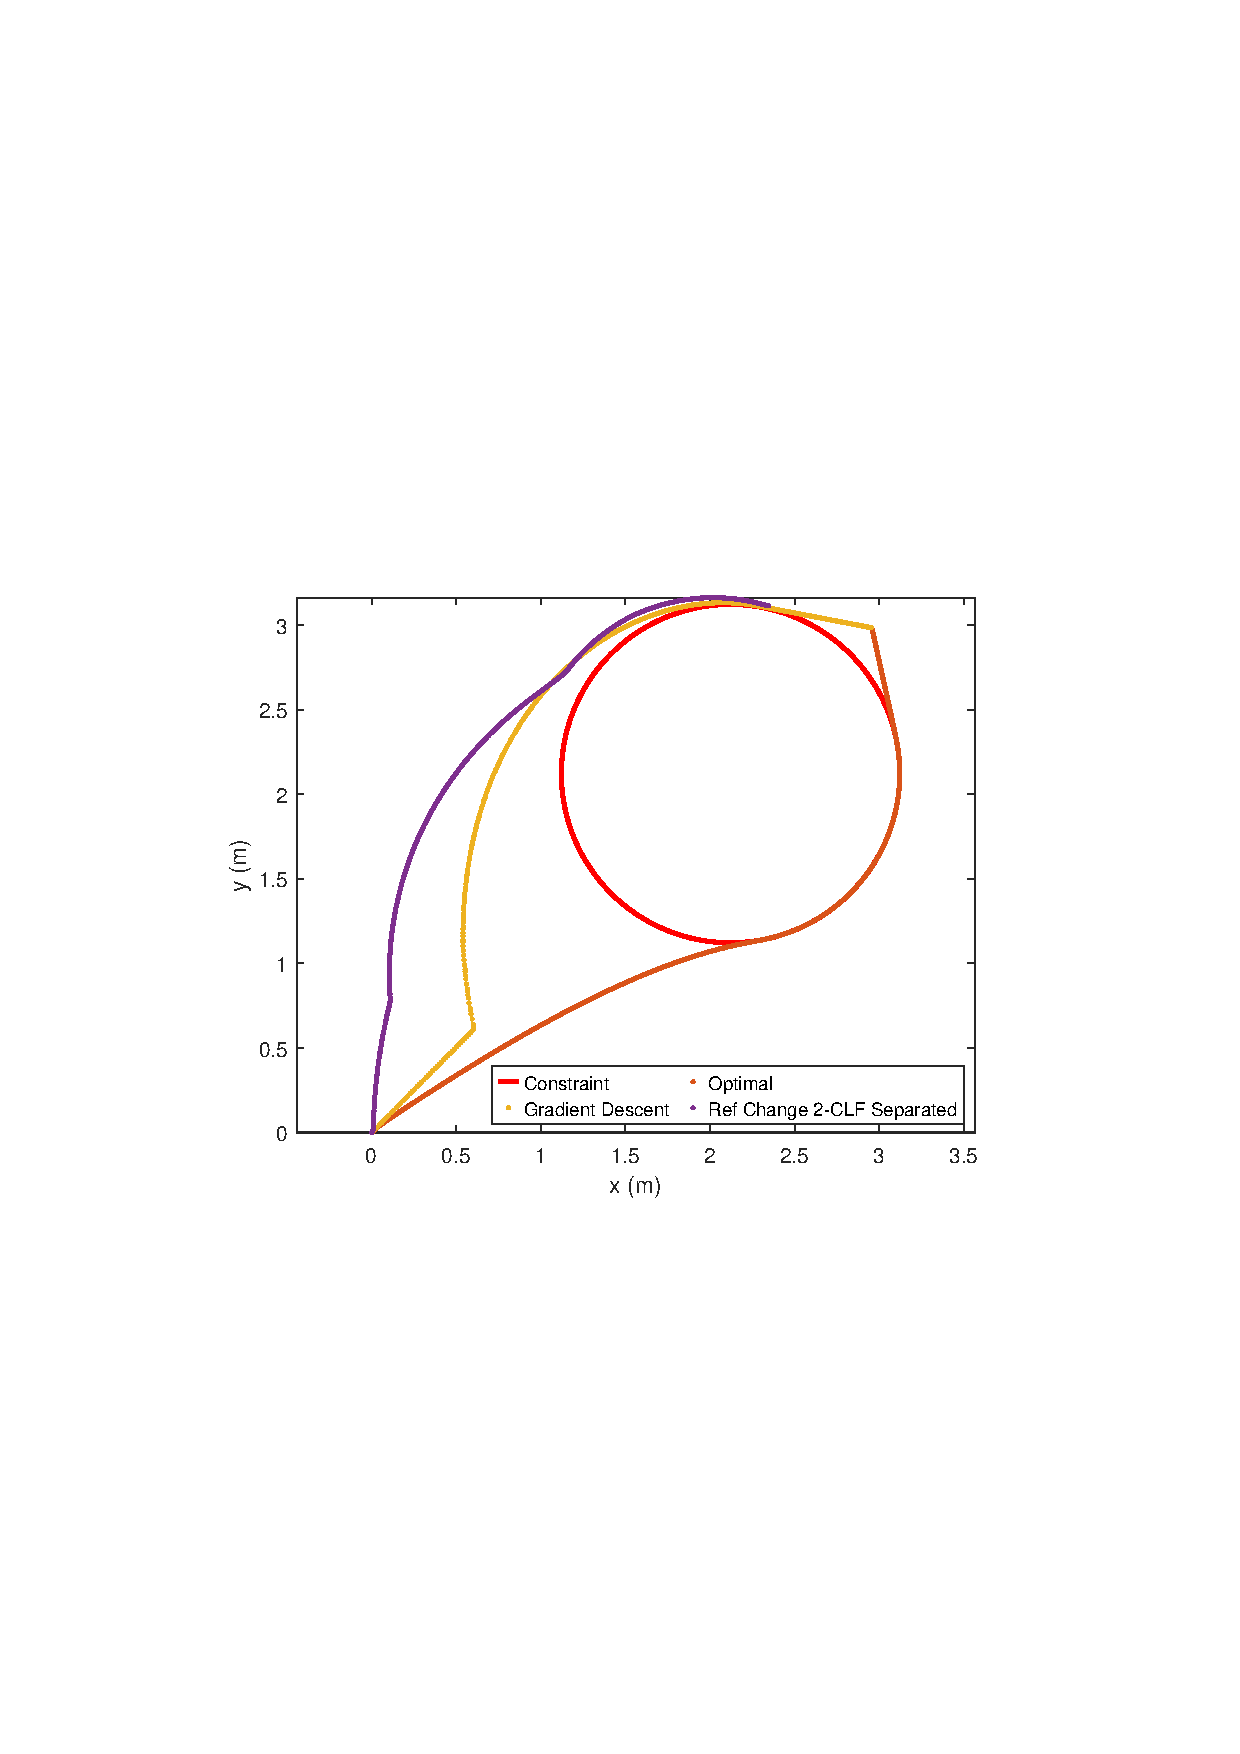
\includegraphics[width=1\linewidth]{UCC.pdf}
  %\caption{A figure with two sub-figures!}
  \label{fig:UCC_CostEvol}
  \end{subfigure}
  \begin{subfigure}{0.6\textwidth}
    \centering
    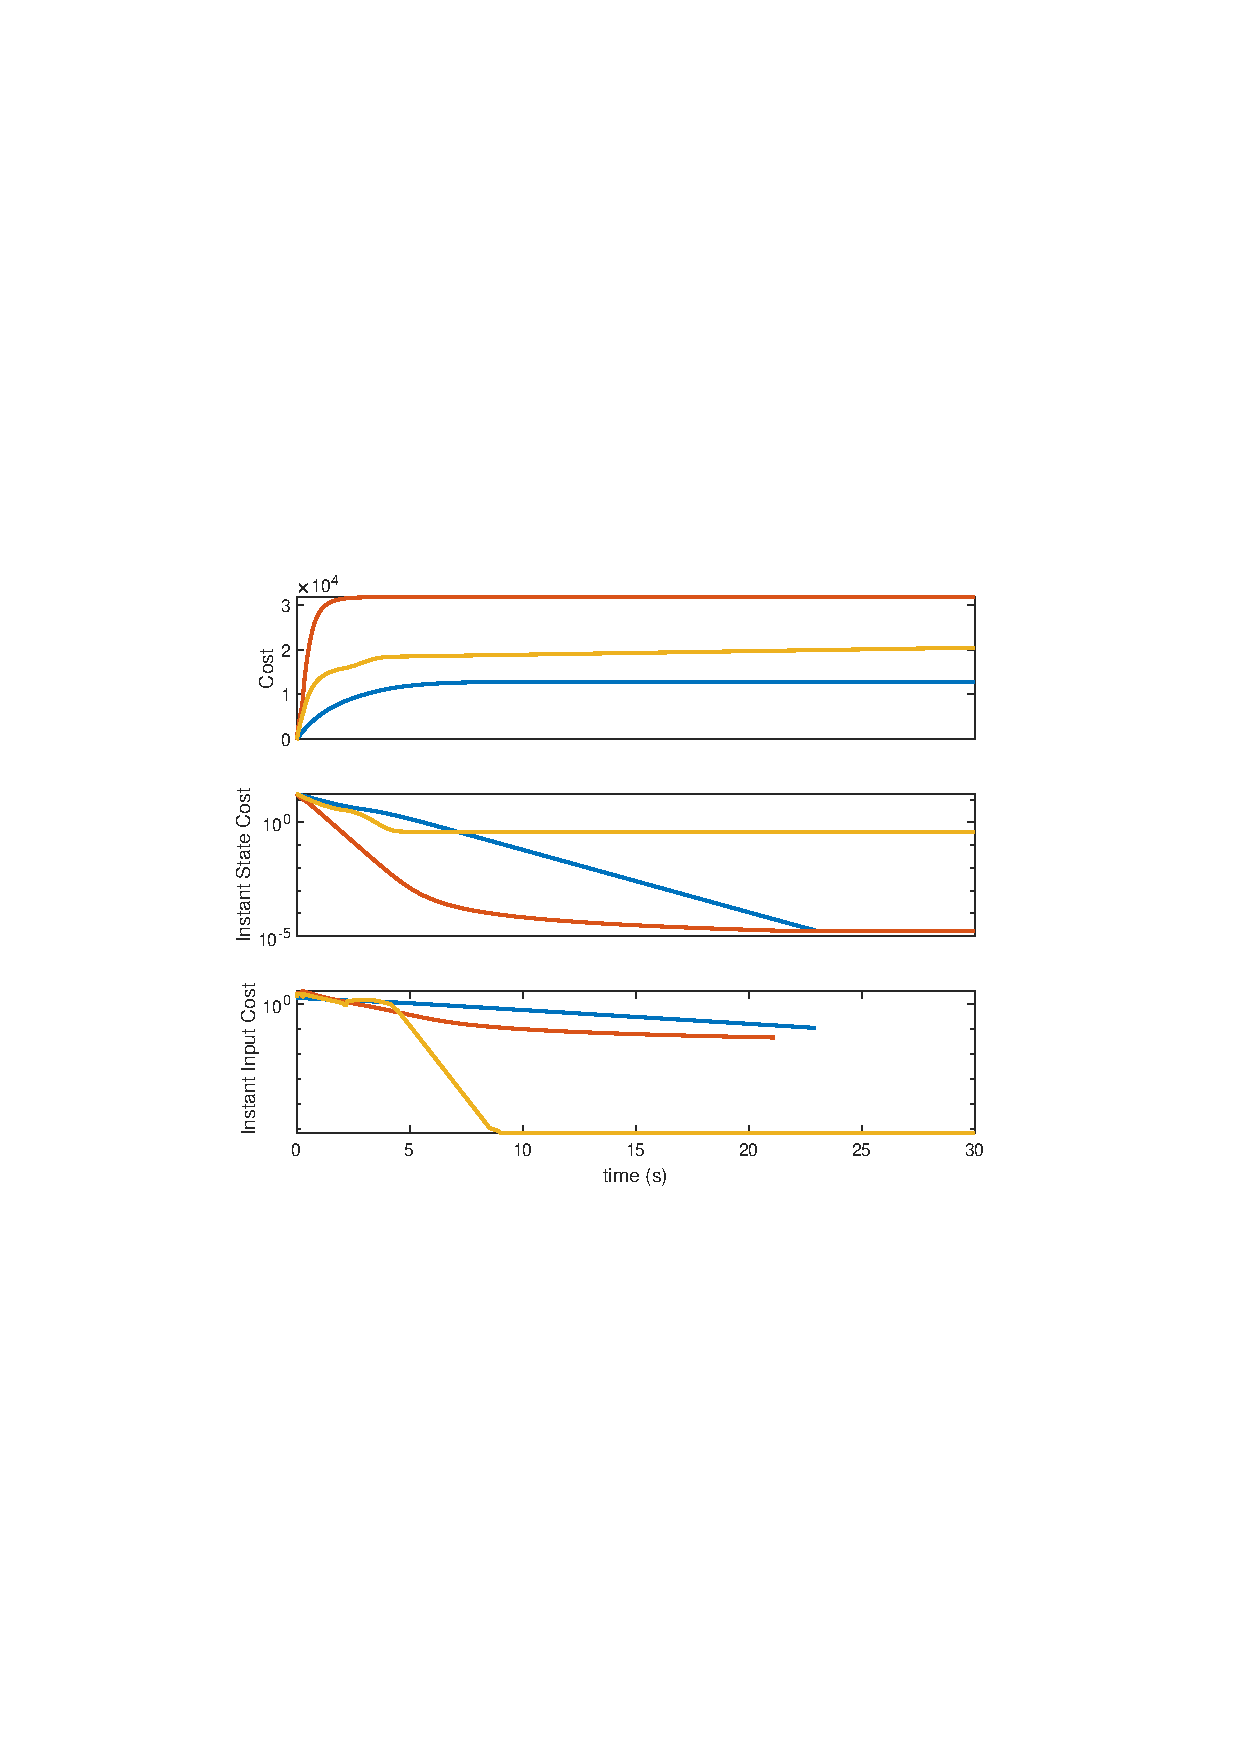
\includegraphics[width=1\linewidth]{UCC_costs.pdf}
  %\caption{A figure with two sub-figures!}
  \label{fig:UCC_trajectory}
  \end{subfigure}
  \caption{UCC~\ref{ssssec:UCC}}
\label{fig:UCCTrajectory_and_CostEvol}
\end{figure}


Although \glsxtrshort{A-JO} \(\alpha\) parameter is optimized its decision keeps beeing purely based on a \glsxtrshort{CLF-CBF} technique which lacks a bigger prediction horizon and thus taking the unicycle close to the obstacle as it is the way that approximates more to the \(\mathbf{ref}\) in the moment (less state cost initially compared to A-CLF-summed), obligating eventually to higher input values to deviate from the barrier safely while forcing as much as possible a speed of convergence to \(\mathbf{ref}\).  The \glsxtrshort{A-CLF-S} following the other point first results in a initially not so fast approximation to \txtref but to a shorter countour path and that allows to avoid abrupt maneuvers leading to less input cost.  

 \newpage %so para ajeiutar


  \bgroup
 \rowcolors{1}{}{orange!4}
 \begin{xltabular}{\textwidth}{|l|cccccc|}
   \toprule
   \rowcolor{blue!6}%
   Algorithms   & DecisionTime & OPtiTime & ReachTime  & InputCost   & StateCost & Cost           \\
   \midrule
    \glsxtrshort{A-JO}~\ref{subsec:Just_Optimized_Algorithm}           & 1.89e-4 & 1.82 & 50 & 282.36 & 7101.2 & 7383.6 \\
    \glsxtrshort{A-CLF-S}~\ref{subsubsec:CLFs_Summed_Algorithm}        & 2.29e-4 & 2.45 & 50 & 352.96 & 5224.5 & 5577.5 \\
    Optimal (\glsxtrshort{MPC} of 6000 horizon)                        & ---     & ---  & 15.65  & 6440  & 6448.8 & 2577.5 \\
    \midrule
    \caption{Some UCC Data}
    \label{tab:Some_UCC_Data}\\
   \end{xltabular}
 \egroup

The \glsxtrshort{A-JO} decion time taked is comparable to a typical \glsxtrshort{CLF-CBF}. It was less time consuming than \glsxtrshort{A-CLF-S} during the experiment and the optimization time too, as it happens an optimization of the \(\alpha\) parameter too along with the computation of the new reference point by \glsxtrshort{A-CLF-S}. The resulting cost of the \glsxtrshort{A-JO} is comparably way higher, as in the next experiments, the trajectories generated by it are longer reflecting particularly in the high input cost and the paths generally more conflicting with the obstacle verifying a greater softening of the \glsxtrshort{CLF} constraint and the presence in more expensive states. \\


\underline{UCF}
\label{ssssec:UCF_experiments} %Unicycle Circular Close Looking


\begin{figure}[htbp]
  \begin{subfigure}{0.55\textwidth}
    \centering
    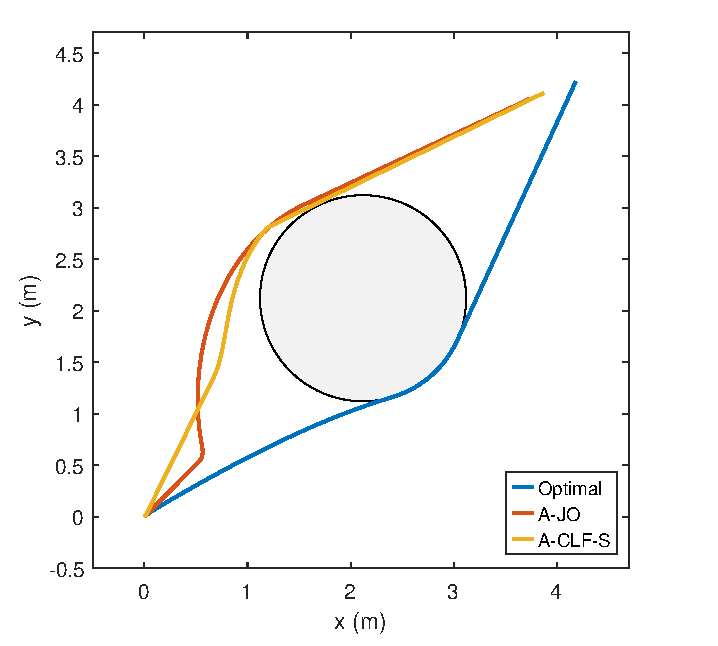
\includegraphics[width=1\linewidth]{UCF.pdf}
  %\caption{A figure with two sub-figures!}
  \label{fig:UCF_CostEvol}
  \end{subfigure}
  \begin{subfigure}{0.6\textwidth}
    \centering
    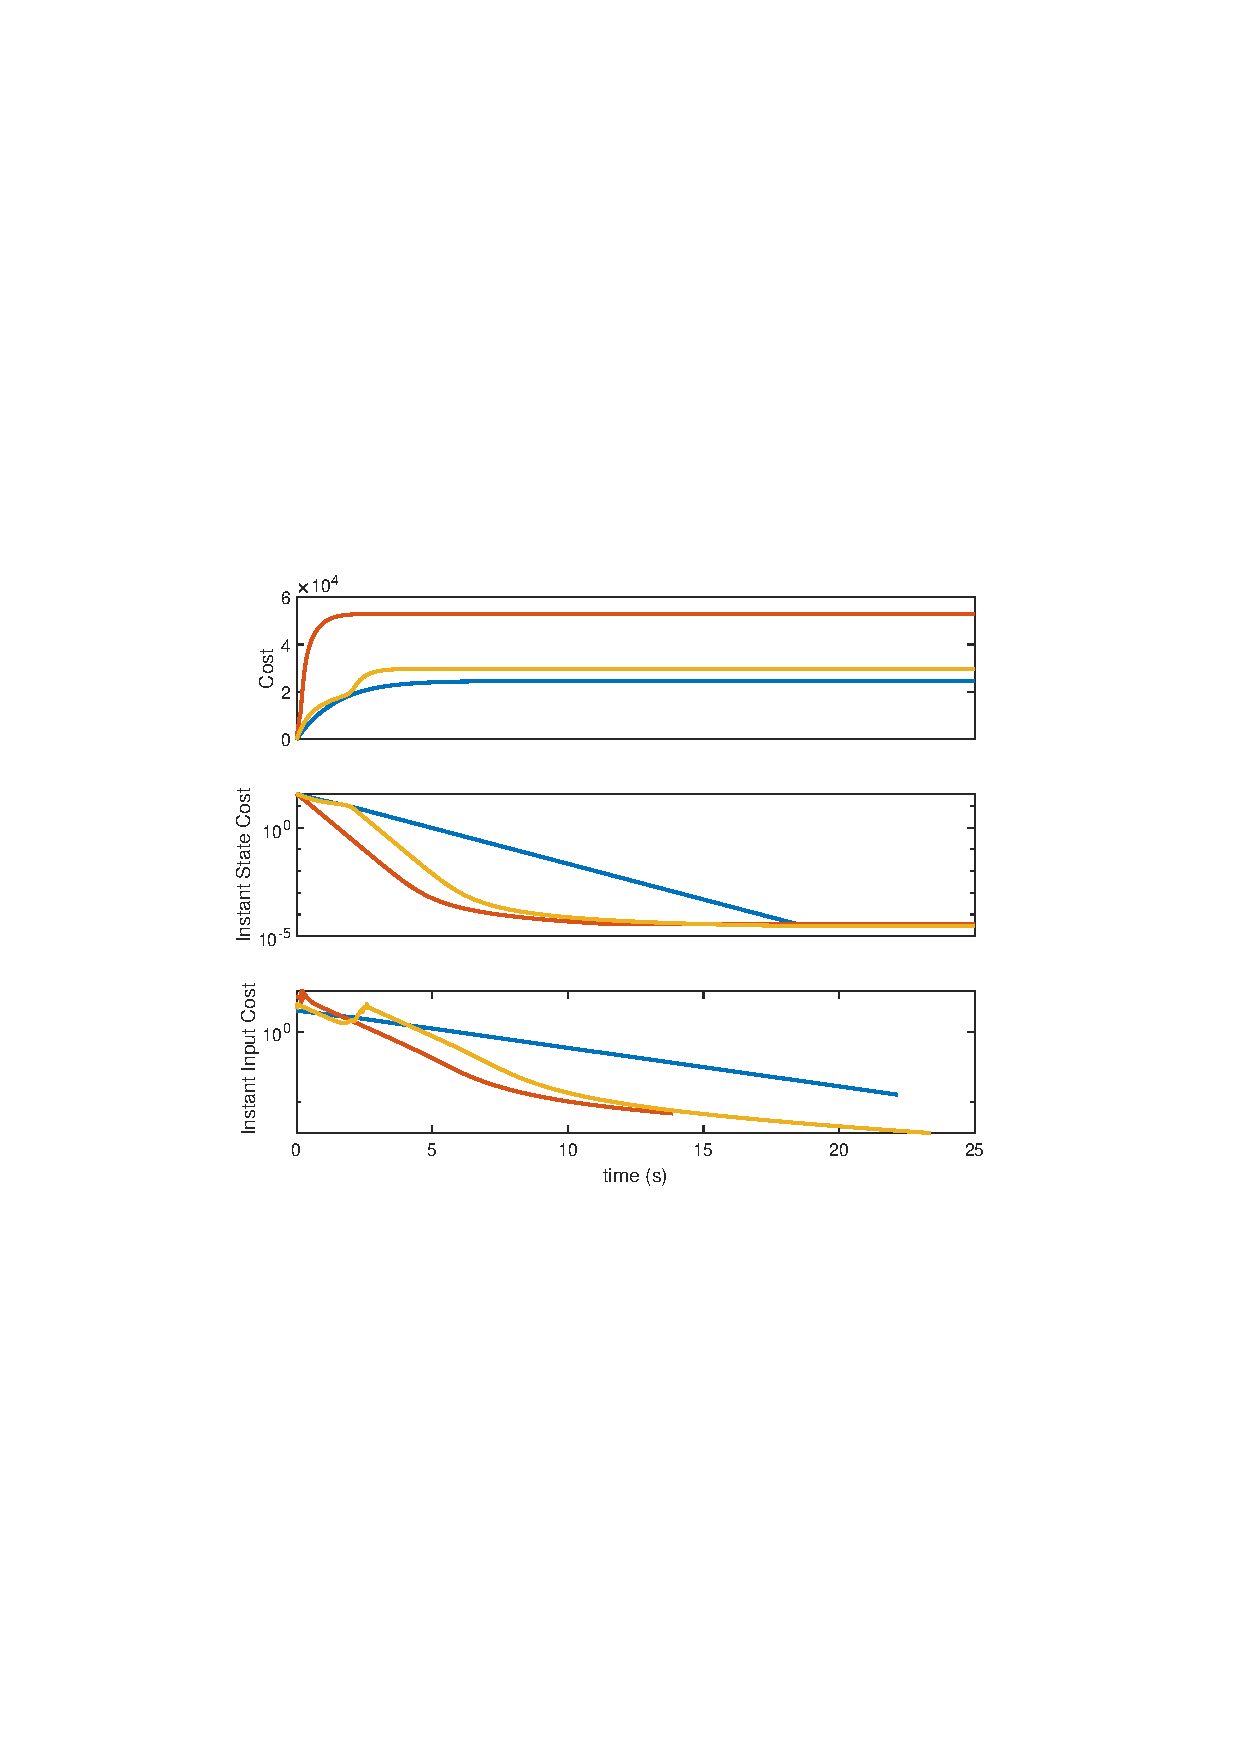
\includegraphics[width=1\linewidth]{UCF_costs.pdf}
  %\caption{A figure with two sub-figures!}
  \label{fig:UCF_trajectory}
  \end{subfigure}
  \caption{UCF~\ref{ssssec:UCF}}
\label{fig:UCFTrajectory_and_CostEvol}
\end{figure}



The \glsxtrshort{A-JO} keeps showing the same characteristics in comparison with \glsxtrshort{A-CLF-S} as it was seen in UCC\ref{ssssec:UCC_experiment}, but in this case is more evident the higher input due to the initial turning of the unicyle and other relative abrupt ones due to the change of convergence point. The \glsxtrshort{A-CLF-S} reveals a relatively similar path to the optimal solution but a slower convergence to \txtref as the \(\gamma\) parameter value (not subject to an optimization) is too low and static, which results in lower inputs but expensive states penalizing in the total cost. \\ 

\vspace{5em}


  \bgroup
 \rowcolors{1}{}{orange!4}
 \begin{xltabular}{\textwidth}{|l|cccccc|}
   \toprule
   \rowcolor{blue!6}%
   Algorithms   & DecisionTime & OPtiTime & ReachTime  & InputCost   & StateCost & Cost           \\
   \midrule
    \glsxtrshort{A-JO}~\ref{subsec:Just_Optimized_Algorithm}           & 1.98e-4 & 2.06 & 50 & 487.21 & 14413 & 14900 \\
    \glsxtrshort{A-CLF-S}~\ref{subsubsec:CLFs_Summed_Algorithm}        & 2.32e-4 & 2.83 & 50 & 1060.5 & 8668.7 & 9729.2 \\
    Optimal (\glsxtrshort{MPC} of 6000 horizon)                        & ---     & ---  & 14.855  & 2465.8  & 2469.4 & 4935.2 \\
    \midrule
    \caption{Some UCF Data}
    \label{tab:Some_UCF_Data}\\
   \end{xltabular}
 \egroup

Even though the input cost of the \glsxtrshort{A-JO} is lower than \glsxtrshort{A-CLF-S}, its sate cost is even more higher. Relative to the computational times, decision and optimization wise the comparation between them keeps the same. \\

 %\newpage %so para ajeiutar

\underline{UEV}
\label{ssssec:UEV_experiments} %Unicycle Ellipse Vertical

 \begin{figure}[htbp]
  \begin{subfigure}{0.5\textwidth}
    \centering
    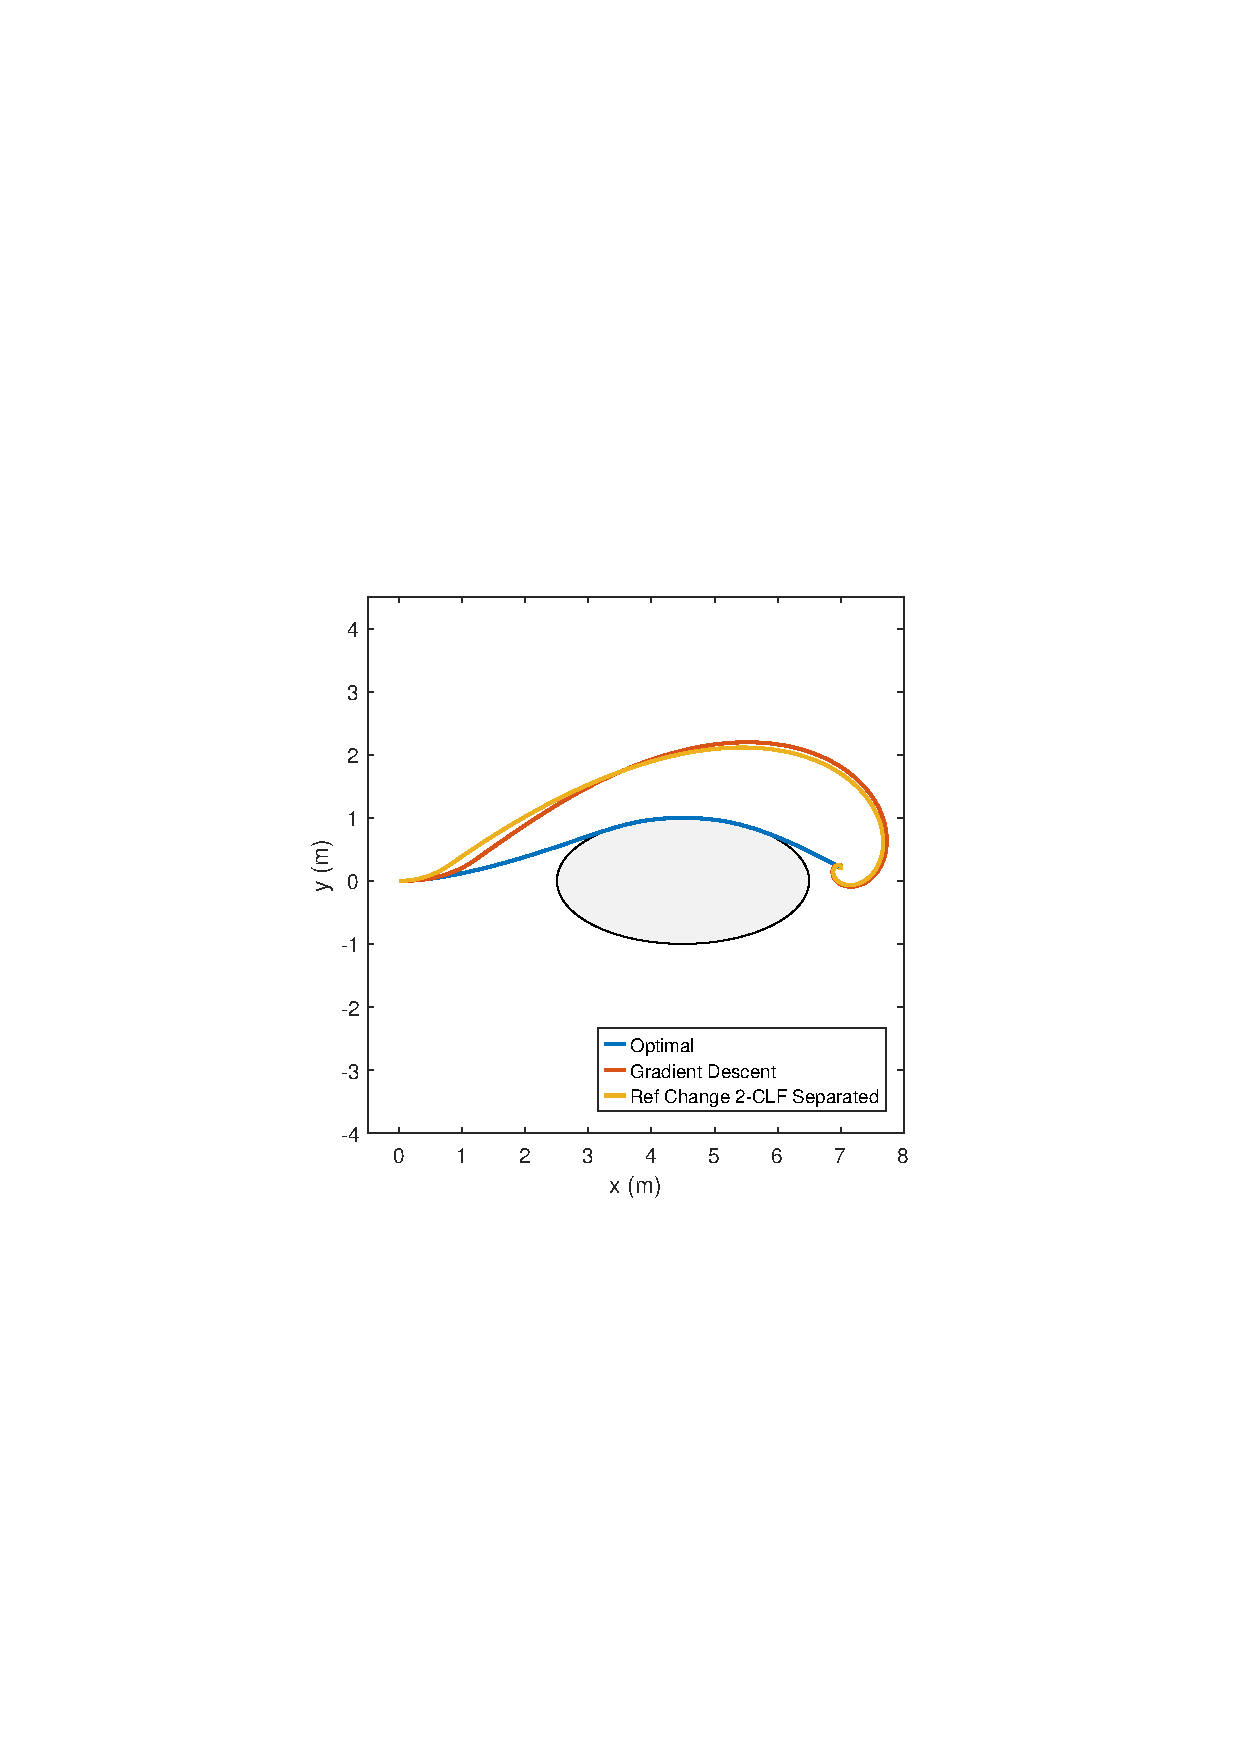
\includegraphics[width=1\linewidth]{UEV.pdf}
  %\caption{A figure with two sub-figures!}
  \label{fig:UEV_CostEvol}
  \end{subfigure}
  \begin{subfigure}{0.6\textwidth}
    \centering
    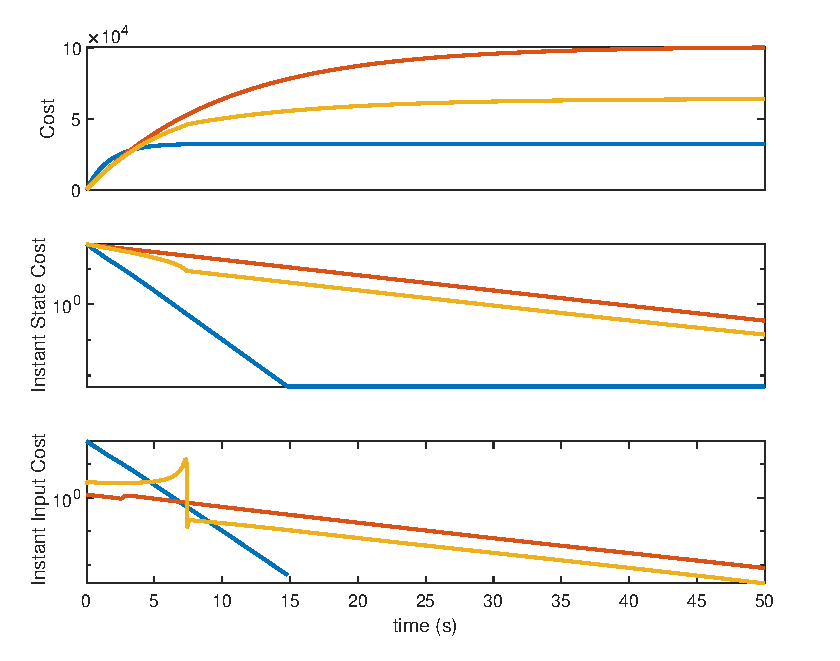
\includegraphics[width=1\linewidth]{UEV_costs.pdf}
  %\caption{A figure with two sub-figures!}
  \label{fig:UEV_trajectory}
  \end{subfigure}
  \caption{UEV~\ref{ssssec:UEV}}
\label{fig:UEVTrajectory_and_CostEvol}
\end{figure}

Now given an ellipsoidal obstacle, with this kind of axis configuration, the bigger the axis is relative to the other one, the less impactful is \glsxtrshort{A-CLF-S}, not only because of the new point demanding a not so relevant maneuver but also because of the respective ellipse \glsxtrshort{CBF} natural imposure of a more soft avoidance. 


  \bgroup
 \rowcolors{1}{}{orange!4}
 \begin{xltabular}{\textwidth}{|l|cccccc|}
   \toprule
   \rowcolor{blue!6}%
   Algorithms   & DecisionTime & OPtiTime & ReachTime  & InputCost   & StateCost & Cost           \\
   \midrule
    \glsxtrshort{A-JO}~\ref{subsec:Just_Optimized_Algorithm}           & 1.86e-4 & 1.90 & 50 & 547.1 & 19495 & 20042 \\
    \glsxtrshort{A-CLF-S}~\ref{subsubsec:CLFs_Summed_Algorithm}        & 2.43e-4 & 2.37 & 50 & 1142.5 & 11604 & 12747 \\
    Optimal (\glsxtrshort{MPC} of 6000 horizon)                        & ---     & ---  & 14.81  & 3229.5  & 3234.4 & 6463.9 \\
    \midrule
    \caption{Some UEV Data}
    \label{tab:Some_UEV_Data}\\
   \end{xltabular}
 \egroup


 \glsxtrshort{A-JO} computational time keeps beeing lower than \glsxtrshort{A-CLF-S} and now for an not so worst cost.


  \newpage %so para ajeiutar


\underline{UEH}
\label{ssssec:UEH_experiments} %Unicycle Ellipse Vertical

 \begin{figure}[htbp]
  \begin{subfigure}{0.5\textwidth}
    \centering
    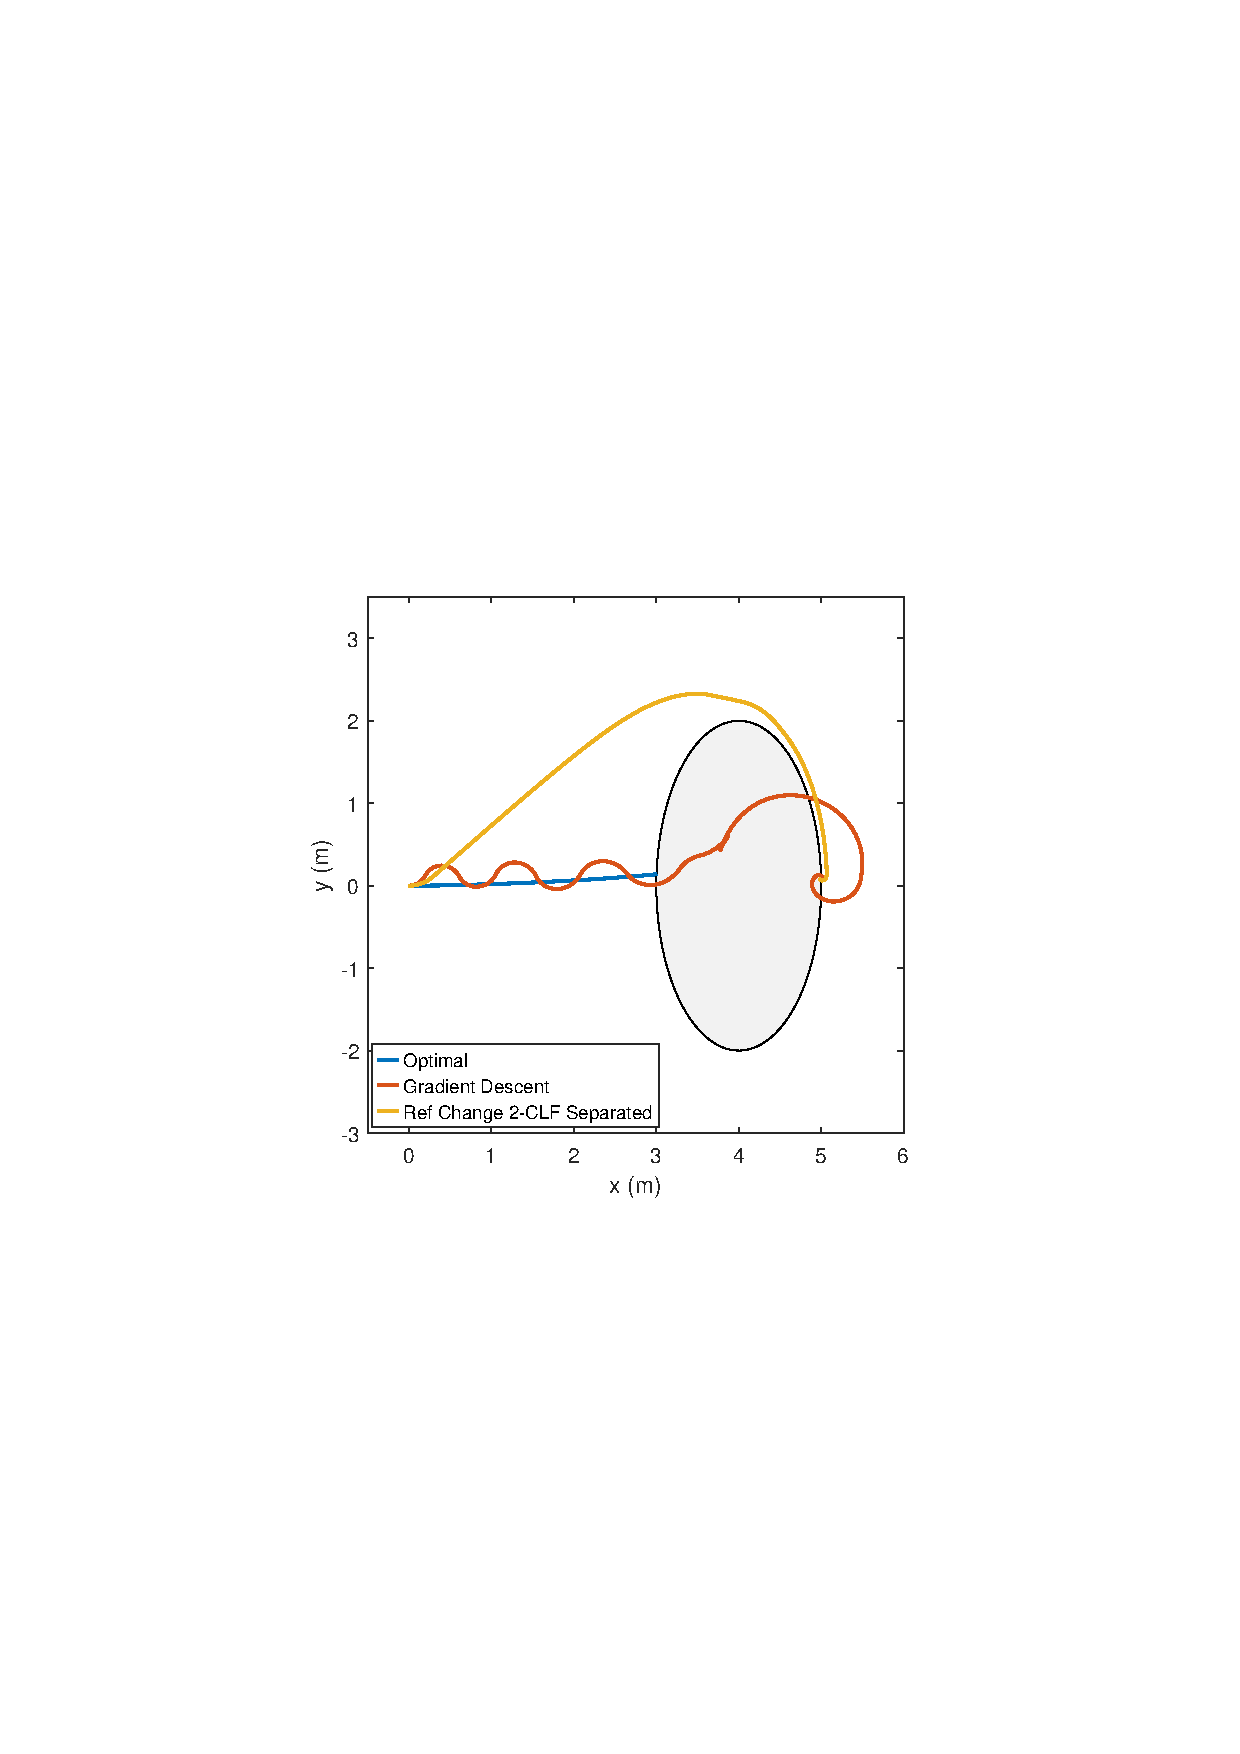
\includegraphics[width=1\linewidth]{UEH.pdf}
  %\caption{A figure with two sub-figures!}
  \label{fig:UEH_CostEvol}
  \end{subfigure}
  \begin{subfigure}{0.6\textwidth}
    \centering
    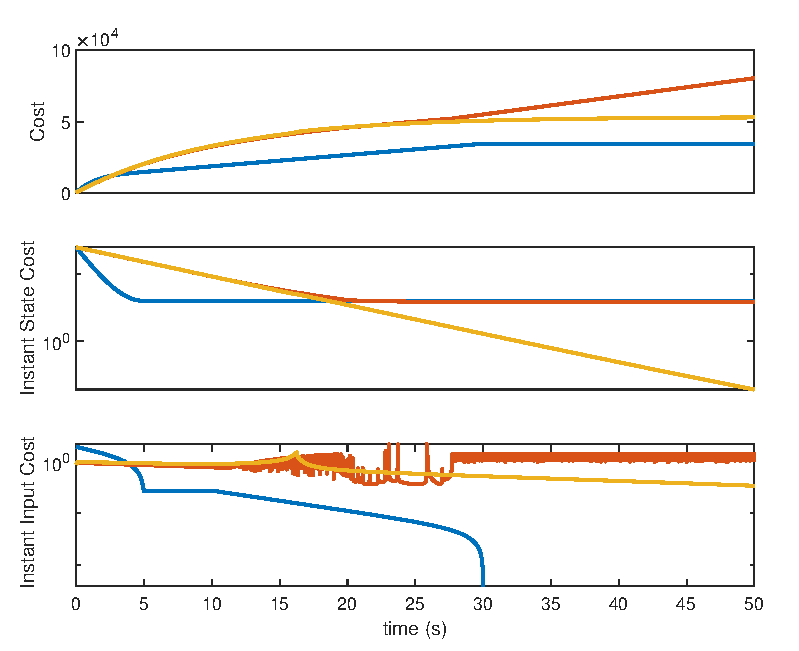
\includegraphics[width=1\linewidth]{UEH_costs.pdf}
  %\caption{A figure with two sub-figures!}
  \label{fig:UEH_trajectory}
  \end{subfigure}
  \caption{UEH~\ref{ssssec:UEH}}
\label{fig:UEHTrajectory_and_CostEvol}
\end{figure}


If in UEV~\ref{ssssec:UEV_experiments} the \glsxtrshort{A-CLF-S} shows a relative worst performance, in this case its path cost is comparatively to it considerably better than \glsxtrshort{A-JO}. Beyond that, important to say that against this type of ellipsoides and orientation againts it and the \txtref, or specially against straight surfaces, the best solution given by the \glsxtrshort{CLF-CBF} is to get the system as close to the obstacle, converging to the its surface, as the \glsxtrshort{CLF-CBF} keeps providing control inputs that lead the system as much closer as possible to the \txtref for each exclusive moment, while the \glsxtrshort{A-CLF-S} converging to the contour point is capable to free from it. The \glsxtrshort{MPC} solution presented corresponds to a local minimum, but its path reveals a similar problem to \glsxtrshort{A-JO} due to the finite horizon and its objective function trying to approximate the system as much to \txtref instead of actually optimize its reaching time, or like \glsxtrshort{A-CLF-S}, although not as effective, make an optimization purely based of the last theoretical state.  


  \bgroup
 \rowcolors{1}{}{orange!4}
 \begin{xltabular}{\textwidth}{|l|cccccc|}
   \toprule
   \rowcolor{blue!6}%
   Algorithms   & DecisionTime & OPtiTime & ReachTime  & InputCost   & StateCost & Cost           \\
   \midrule
    \glsxtrshort{A-JO}~\ref{subsec:Just_Optimized_Algorithm}           & 1.92e-4 & 1.92 & 50 & 2958.5 & 13435  & 16394 \\
    \glsxtrshort{A-CLF-S}~\ref{subsubsec:CLFs_Summed_Algorithm}        & 2.52e-4 & 2.73 & 50 & 574.53 & 10007 & 10582  \\
    Optimal (\glsxtrshort{MPC} of 6000 horizon)                        & ---     & ---  & 50  & 1053.9  & 9015.4 & 10069 \\
    \midrule
    \caption{Some UEH Data}
    \label{tab:Some_UEH_Data}\\
   \end{xltabular}
 \egroup

 %\vspace{5em}

 The cost don't necessarily means a better performance. As it is possible to see, the \glsxtrshort{A-CLF-S} is the only one of the them beeing able to surpass the obstacle although its cost is the lower.

\begin{tcolorbox}[colback=blue!5!white,colframe=blue!35!white,title=Notes:]
\begin{itemize}
    \item If the constraint is circular and the vehicle is oriented to the \txtref and to the center of the circle, the unicycle converges to the obstacle limit.
  \end{itemize}
\end{tcolorbox} 

\newpage %so para ajeitar

\underline{UED}
\label{UED_experiments} %Unicycle Ellipse Vertical

 \begin{figure}[htbp]
  \begin{subfigure}{0.5\textwidth}
    \centering
    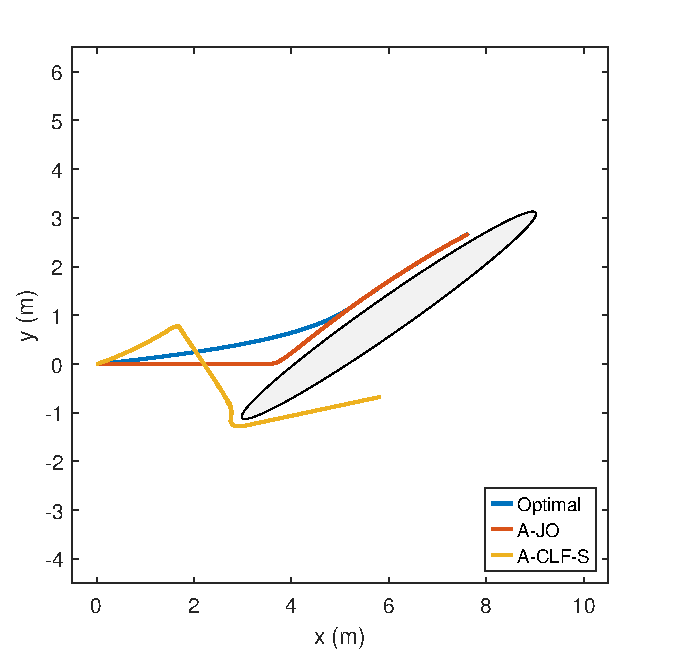
\includegraphics[width=1\linewidth]{UED.pdf}
  %\caption{A figure with two sub-figures!}
  \label{fig:UED_CostEvol}
  \end{subfigure}
  \begin{subfigure}{0.6\textwidth}
    \centering
    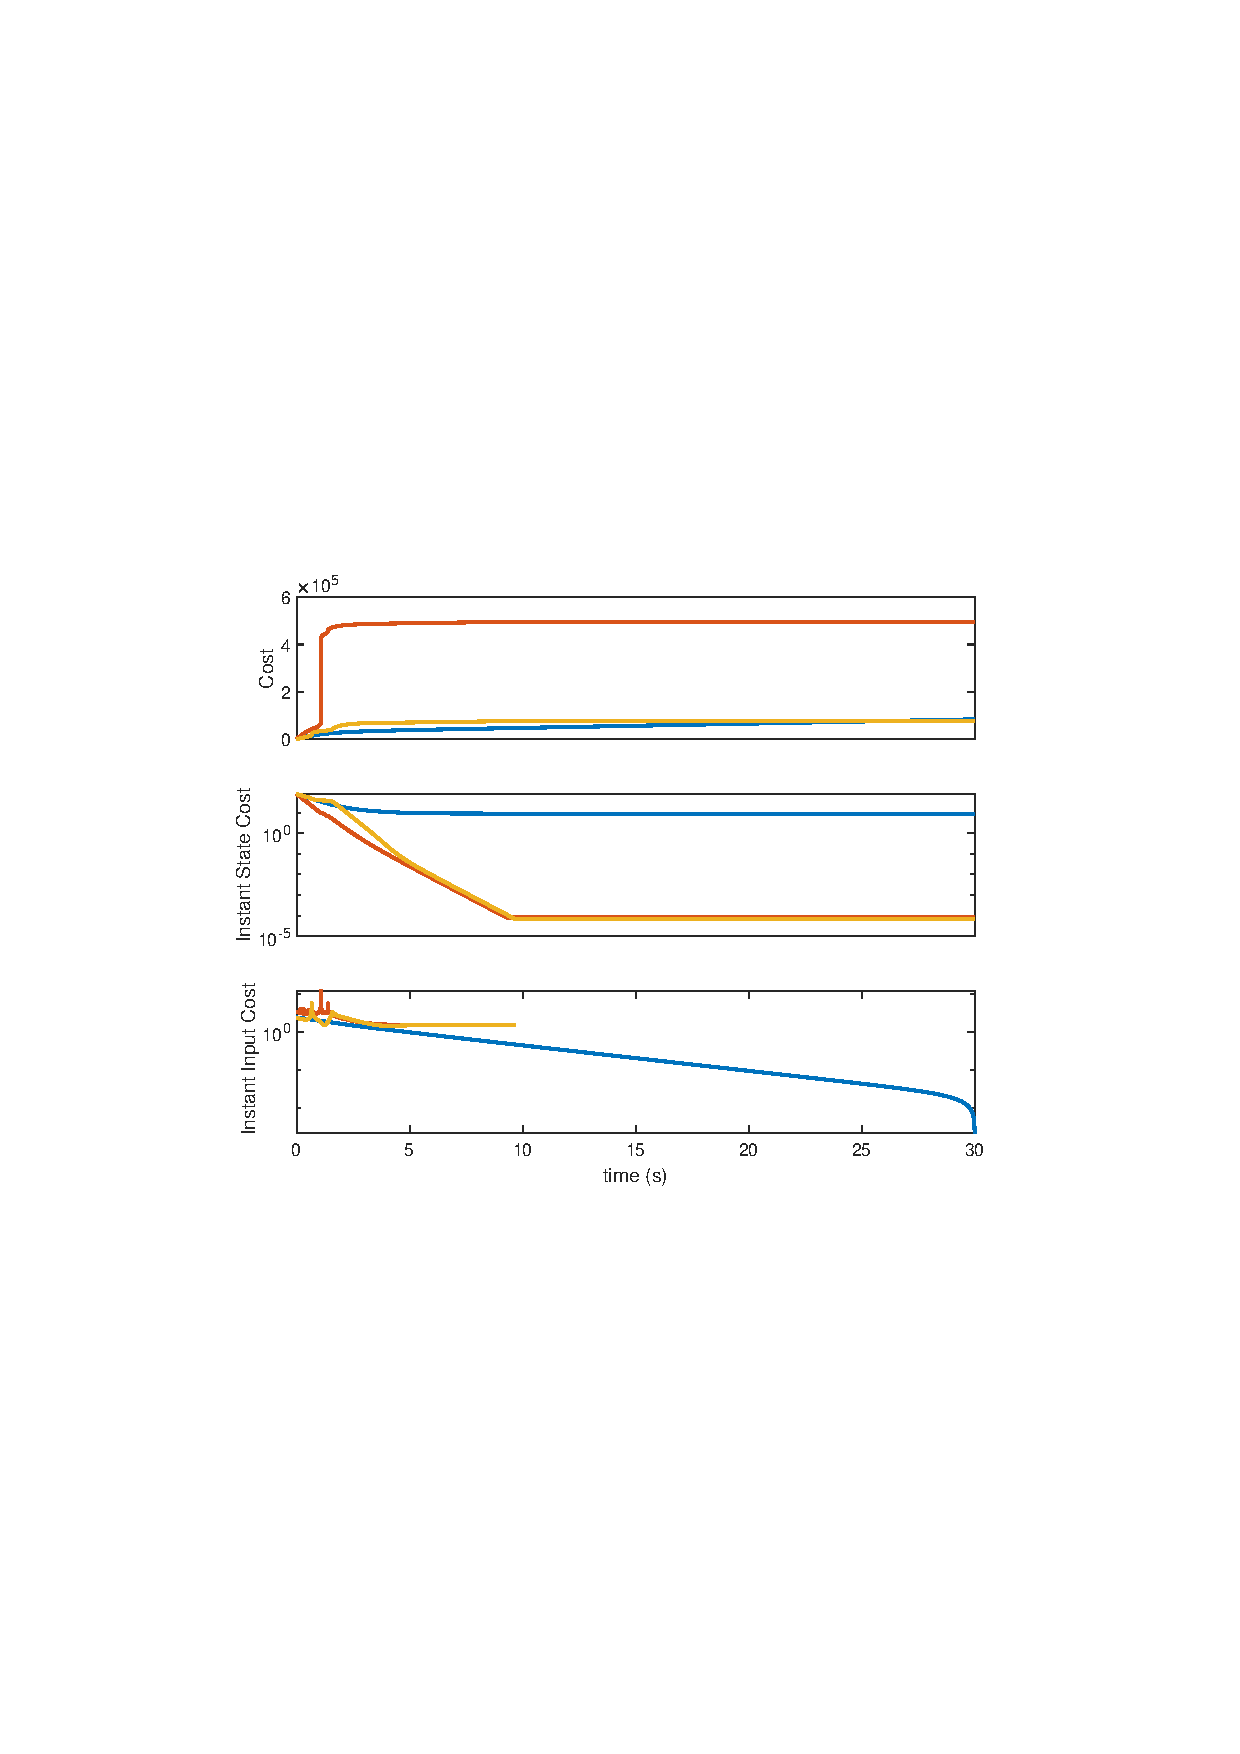
\includegraphics[width=1\linewidth]{UED_costs.pdf}
  %\caption{A figure with two sub-figures!}
  \label{fig:UED_trajectory}
  \end{subfigure}
  \caption{UED~\ref{ssssec:UED}}
\label{fig:UEDTrajectory_and_CostEvol}
\end{figure}


As in UEH~\ref{ssssec:UEH_experiments}, although the other techiniques don't keep stuck, they keep the same characteristics and go for the longest side. While the \glsxtrshort{A-CLF-S} keeps showing a better result.


  \bgroup
 \rowcolors{1}{}{orange!4}
 \begin{xltabular}{\textwidth}{|l|cccccc|}
   \toprule
   \rowcolor{blue!6}%
   Algorithms   & DecisionTime & OPtiTime & ReachTime  & InputCost   & StateCost & Cost           \\
   \midrule
    \glsxtrshort{A-JO}~\ref{subsec:Just_Optimized_Algorithm}           & 2.1e-4 & 2.12 & 50 & 9769.6 & 38910  & 48680 \\
    \glsxtrshort{A-CLF-S}~\ref{subsubsec:CLFs_Summed_Algorithm}        & 3.18e-4 & 3.58 & 50 & 11497 & 77575 & 89073  \\
    Optimal (\glsxtrshort{MPC} of 6000 horizon)                        & ---     & ---  & 50  & 4243 & 22267 & 26510 \\
    \midrule
    \caption{Some UED Data}
    \label{tab:Some_UED_Data}\\
   \end{xltabular}
 \egroup


\subsection{Orbital}
\label{subsec:orbital_experiments}

-mostrar as simulaçoes\\
-explicar os resultados obtidos

















% Most latex users will instead create more and more advanced commands.
% A lot of us have a "commands.tex" that we "\input{commands.text}" at the beginning of all our documents.
% Taking simple examples, I have \newcommand{\CC}{\mathbb{C}} at part of the commands in most of my documents because I use the field of complex number everywhere and \CC is shorter to write than \mathbb{C}. I also have \newenvironment{ctabular}[1]{\begin{center}\begin{tabular}{#1}}{\end{tabular}\end{center}} for whenever I need a centred tabular, which is almost always.

% \makeatletter %Transforma o @ para um caracter normal
% \newcommand{\ntifpkgloaded}{%
%   \@ifpackageloaded% %Não esta ai mas seria mais 3 argumentos {}{}{} o primeiro o package, o segundo e o terceiro if e if not o package tiver sido load respetivamente
% }
% \makeatother %Transforma o @ para um caracter especial outra vez

% \lipsum[1-3]

% \begin{figure}[htbp]
%   \centering
%   \subbottom[One sub-figure\label{fig:leftsubfig}]{%
%     
\includegraphics[width=0.5\linewidth]{knitting-vectorial}}%
%   \subbottom[Another sub-figure\label{fig:rightsubfig}]{%
%     
\includegraphics[width=0.5\linewidth]{knitting-vectorial}}%
%   \caption{A figure with two sub-figures!}
%   \label{fig:fig2subfig}
% \end{figure}



%  The Table~\ref{tab:hla:results} illustrates some important concepts associated with table construction:
%  \begin{asparaenum}[i)]
%  \item Do not use vertical lines;
%  \item The caption should be above the table;
%  \item Use the macros \verb!\toprule!, \verb!\midrule! and \verb!\bottomrule! to make the top, inner and bottom horizontal lines, respectively.
%  \end{asparaenum}

%  \bgroup
%  \rowcolors{1}{}{GhostWhite}
%  \begin{xltabular}{\textwidth}{Xccccc}
%    \caption{Test results summary.}
%    \label{tab:hla:results}\\
%    \toprule
%    \rowcolor{Gainsboro}%
%    Test   & Anomalies  & Warnings  & Correct   & Categories            & Missed \\
%    \midrule
%  Connection~\cite{Beckman08}     & 2       & 2          & 1          & \emph{C}              & 1 \\
%  Coordinates'03~\cite{Artho03}   & 1        & 4          & 1          & \emph{2B, 1C}          & 0 \\
%  Local Variable~\cite{Artho03}    & 1        & 2          & 1          & \emph{A}              & 0 \\
%  NASA~\cite{Artho03}              & 1        & 1          & 1          & ---                    & 0 \\
%    \midrule
%    \rowcolor{Gainsboro}%
%  Total                            & 12      & 33        & 10        & 5A, 6B, 10C, 2D       & 2 \\
%    \bottomrule
%    \end{xltabular}
%  \egroup


%  \begin{figure}[htbp]
%    \centering
%    
\includegraphics[height=1in]{snowman-vectorial}
%    
\includegraphics[height=3in]{snowman-vectorial}
%    
\includegraphics[height=6in]{snowman-vectorial}
%    \caption{Vectorial image (PDF)}
%    \label{fig:Figures_Tree_silhouettes-vectorial}
%  \end{figure}

% To combine several figures into a single one… You can then reference the set as Figure~\ref{fig:complete-figure} or the sub-figures separately as~\ref{fig:woolball} and~\ref{fig:cloud}.

% \begin{figure}[htbp]
%   \centering
%     \subbottom[Novelo de lã]{%
%     \label{fig:woolball}
%     
\includegraphics[height=1in]{knitting-vectorial}
%     }
% \qquad\qquad
%     \subbottom[Tempestade com neve]{%
%     \label{fig:cloud}
%     
\includegraphics[height=1in]{snowstorm-vectorial}
%     }
%   \caption{Exemplo de utilização de \emph{subbottom}}
%   \label{fig:complete-figure}
% \end{figure}


% Uncomment the algorithms source below and add the following to file “\verb!5_packages.tex!”
% \begin{verbatim}
%   \usepackage{algorithm2e}
%   \RestyleAlgo{ruled}
% \end{verbatim}
% and uncomment
% \begin{verbatim}
% \ntaddlistof{listofalgorithms}
% \end{verbatim}
% in file “\verb!8_list_og.tex!”.



%NÂO CONSEGUI POR A FUNCIONAR MAS OLHEI POUCO

% \newif\ifntlistingsloaded
% \ntifpkgloaded{listings}{\ntlistingsloadedtrue}{\ntlistingsloadedfalse}
% \newif\ifntmintedloaded
% \ntifpkgloaded{minted}{\ntmintedloadedtrue}{\ntmintedloadedfalse}

% \ifntlistingsloaded
% \section{Test for listings} % (fold)
% \label{sec:test_for_listings}

% Testing the package “listings“…

% \begin{lstlisting}[caption=cap,label=lst:lab,float=htbp]
% if(a==b)
%   puts("YESS!")
% \end{lstlisting}
% \fi

% \ifntmintedloaded
% \section{Test for minted} % (fold)
% \label{sec:test_for_minted}

% Testing the package “minted“…

% \begin{listing}[H]
%   \begin{minted}{C}
%     if(a==b)
%       puts("YESS!")
%   \end{minted}
%   \caption{Example of a listing.}
%   \label{lst:lab}
% \end{listing}
% \fi
